\documentclass[11pt]{article}
\usepackage[utf8]{inputenc}	% Para caracteres en español
\usepackage{amsmath,amsthm,amsfonts,amssymb,amscd}
\usepackage{fullpage}
\usepackage{setspace}
\usepackage[margin=3cm]{geometry}
\usepackage[hidelinks]{hyperref}

\usepackage{bm}
\usepackage{cleveref}
\usepackage{graphicx}
\usepackage{algpseudocode}
\usepackage{algorithm}
\usepackage{algorithmicx}
\usepackage{booktabs}
\usepackage{todonotes}

\setlength{\fboxsep}{0.05\textwidth}

\newcommand{\commentEq}[1]{%
  \text{\phantom{(#1)}} \tag{#1}
}
\geometry{margin=1in, headsep=0.25in}

\begin{document}
\setcounter{section}{0}
\thispagestyle{empty}

\noindent\fbox{\begin{minipage}{0.9\textwidth}
  \begin{center}
    \section*{CS 7140: Advanced Machine Learning}
	\subsection*{Project Report:  Weight Uncertainty in Neural Networks}
  \end{center}
  
  \noindent\textbf{Instructor}
  \smallskip
  
  Jan-Willem van de Meent (\url{j.vandemeent@northeastern.edu})\\
  
  \noindent\textbf{Students}
  \smallskip

  Colin Kohler (\url{kohler.c@husky.neu.edu})\\
  Andrea Baisero (\url{baisero.a@husky.neu.edu})
\end{minipage}}
\bigskip

\newcommand\Ind{{\mathbb{I}}}
\newcommand\Exp{{\mathbb{E}}}
\newcommand\KL{{\operatorname{KL}}}

\section{Introduction}
A well known problem with artificial netural networks is their tendency to 
overfit their training data. This overfitting results in a extremely low 
error on the training data and a large error on the test data. More concretely,
we can state that the network has become overly confident about the amount of
uncertainty in the training data and therfor makes predictions on the test
data which are unrealisticly optimistic. The main method used to combat 
this problem is known as regularization. 

The most naive method of regularization is known as early stopping which simply
involves stopping the network's training once the test error has begun to
increase. More complex forms of regularization involve modifying the loss 
function by adding a penalty term. Through the addition of this penalty, the
network is forced to learn a more general model of the data thereby avoiding
overfitting. In this report we will implement and test a regularization 
technique known as \textit{Bayes by Backprop}~\cite{blundell} which utilizes 
variational Bayesian learning to introduce uncertainty on the weights of the 
neural network.

\subsection{Artificial Neural Networks}
Before discussing Bayes by Backprop, we must take a slight deviation from
the norm to view neural networks (NN) in a more probablistic manner. A neural 
network is typically viewed as a collection of connected units, each with 
their own weight, which takes some input signal and produces an output
signal by passing it through these units. Learning is then acheived by 
using gradient descent to optimize these weights with respect to some loss
function. 

We will formalize this notition by defining a neural network as a probablistic
model, $P(y|x,w)$ where $x \in \mathbb{R}^P, y \in \mathcal{Y}$. Using this 
model, we can view neural networks as a function which assigns a probability
to each possible outcome $y$ given some input $x$ through the use of the set
of weights $w$. These weights are still learned through the use of gradient 
descent however we can now view this learning as the maximum likelihood 
estimate (MLE) of the weights given some data $D=(X,Y)$:
\begin{align*}
  w^{MLE} &= \arg\max_w \log P(D|w) \\ 
  &= \arg\max_w \sum_i \log P(y_i|x_i, w) 
\end{align*}

As Bayes by Backprop is a regularization technique, we have to expand upon this
estimate to include regularization. This is done by introducing a prior on the
weights $w$ and then finding the maximum a posteriori (MAP) weights:
\begin{align*}
  w^{MAP} &= \arg\max_w \log P(w|D) \\
  &= \arg\max_w \log P(D|w) + \log P(w) 
\end{align*}
Depending on the distribution of the prior placed on $w$ we can get different
types of regularization. If $P(w)$ is a gaussian, then we will have L2 
regularization, which is also known as weight decay. If $P(w)$ is a
Laplace distribution, then we will have L1 regularization.


\subsection{Variational Inference}

% Variational Inference (VI) indicates a family of optimization-based inference
% methods which work by approximating the true conditional probability of the
% variables of interest with a

Let $P(\bm y, \bm z)$ denote a generative model of joint observed variables
$\bm y$ and latent variables $\bm z$, and let the conditional distribution
$P(\bm z\mid \bm y)$ be the target of the inference.  Variational inference
(VI)~\cite{blei_variational_2017} indicates a family of optimization-based
methods which approximate the target distribution with a parameterized model
$q(\bm z; \theta)$ known as the \emph{variational} approximation. In VI, the
inference process is driven by the minimization of the Kullback-Leibler (KL)
divergence between the variational approximation and the target conditional,
%
\begin{align}
  %
  \theta^* &= \arg\min_\theta \KL\left( q(\bm z; \theta) \mid\mid P(\bm z\mid
  \bm y) \right) \\
  %
  % &= \arg\min_\theta \KL\left( q(\bm z; \theta) \mid\mid P(\bm z) \right)
  % + \Exp_{q(\bm; \theta)}\left[ -\log P(\bm y\mid \bm z) \right] \\
  %
  &= \arg\min_\theta \Exp_{q(\bm z; \theta)}\left[ \underbrace{ \log q(\bm z;
  \theta) - \log P(\bm z) -\log P(\bm y\mid \bm z) }_{f(\bm y, \bm z; \theta)}
  \right] \label{eq:VI}
  %
\end{align}

\todo[inline]{Maybe define ELBO more explicitly?}

To further simplify the inference process, the variational model is often
designed to satisfy the mean-field assumption, by which each individual latent
variable is modeled independently $q(\bm z; \theta) = \prod_k q(\bm z_k;
\theta_k)$.  With the mean-field assumption in place, and when the joint
generative model and the variational approximation satisfy certain (non-mild)
conjugacy conditions, the VI objective in \cref{eq:VI} can be optimized very
efficiently via a sequence of analytical updates on the variational parameters.

\paragraph{Stochastic Variational Inference}  Depending on the amount data
which is available or required for the model at hand, it may be more efficient
(or necessary) to use a stochastic optimization approach, whereby only
a randomly selected subset of the variational parameters are updated at any
given iteration; this is called Stochastic Variational Inference
(SVI)~\cite{hoffman_stochastic_2013}.

\paragraph{Black Box Variational Inference}  Black Box Variational Inference
(BBVI)~\cite{ranganath_black_2014} is a further extension to addresses the
variational inference minimization problem problem when the conjugacy
conditions are not satisfied.  In such a situation, it is not possible to
derive precise analytical updates on the variational parameters.  Instead, BBVI
uses the gradients of the ELBO to update the parameters using (Stochastic)
Gradient Descent.

\subsection{Gradient Estimation}

BBVI requires the differentiation of an objective in the form of an expectation
whose distribution is itself dependent on the differentiation variables.  While
it is generally possible to estimate the gradient of such an expectation using
the likelihood ratio trick~\cite{williams_simple_1992} (a.k.a. REINFORCE)
followed by Monte Carlo estimation,
%
\begin{align}
  %
  \nabla_\theta \Exp_{q(\bm z;\theta)}\left[ f(\bm y, \bm z; \theta) \right] &=
  \Exp_{q(\bm z;\theta)}\left[ \nabla_\theta \log q(\bm z;\theta) f(\bm y, \bm
  z; \theta) + \nabla_\theta f(\bm y, \bm z; \theta) \right] \nonumber \\
  %
  &\approx \frac{1}{S} \sum_{s=1}^S \nabla_\theta \log q(\bm z_s; \theta) f(\bm
  y, \bm z_s; \theta) + \nabla_\theta f(\bm y, \bm z_s; \theta) \,, \bm z_s
  \sim q(\bm z; \theta)
  %
\end{align}
%
\noindent the resulting estimate has a high variance due to the \emph{score}
function $\nabla_\theta \log q(\bm z; \theta)$ being roughly inversely
proportional to the sampling likelihood $q(\bm z; \theta)$, and is thus
substantially less-than-ideal for the purpose of performing gradient descent.

\paragraph{Reparameterization Trick}

The reparameterization trick is an algebraic manipulation which simplifies the
differentiation and avoids introducing the score function, which is the source
of the high variance in REINFORCE.  The reparameterization is available
whenever it is possible to reformulate the process of sampling from the
proposal distribution $\bm z\sim q(\bm z; \theta)$ as a deterministic function
$\bm z(\epsilon; \theta)$ of an independently sampled auxiliary variable
$\epsilon\sim p(\epsilon)$.  Applying this substitution, the expectation
distribution becomes independent from the differentiation parameters, meaning
that the differentiation operator can move inside the expectation unscattered:
%
\begin{align}
  %
  \nabla_\theta \Exp_{q(\bm z; \theta)}\left[ f(\bm y, \bm z; \theta) \right] &=
  \nabla_\theta \Exp_{p(\epsilon)}\left[ f(\bm y, \bm z(\epsilon; \theta); \theta) \right] \nonumber \\
  %
  &= \Exp_{p(\epsilon)}\left[ \nabla_\theta f(\bm y, \bm z(\epsilon; \theta); \theta) \right] \nonumber \\
  %
  &\approx \frac{1}{S} \sum_{s=1}^S \nabla_\theta f(\bm y, \bm z(\epsilon_s; \theta); \theta)\,, \epsilon_s \sim p(\epsilon)
  %
\end{align}

\section{Bayes by Backprop} \label{sec:bayes_by_backprop}

The authors propose to use variational inference to obtain a Bayesian treatment
of neural networks.  The latent variables of a NN architecture are its weights
$w$, and the chosen variational approximation models them with independent
Normal distributions;  thus the variational parameters represent the Normal
means $\mu$ and standard deviations $\sigma$---the latter is represented
indirectly by a parameter $\rho$, which is then passed through the softplus
function to guarantee positiveness:
%
\begin{align}
  %
  \theta &= \{ \mu, \rho \} \\
  %
  \sigma &= \log(1 + \exp\rho) \\
  %
  q(w_k; \theta) &= \mathcal{N}(w_k; \mu_k, \sigma_k^2)
  %
\end{align}

\todo[inline]{Talk about prior!}

The Normal distribution lends itself very naturally to a simple form of
reparameterization meaning that we can exploit the reparameterization trick to
compute better gradient estimates:
%
\begin{align}
  %
  \epsilon_k &\sim \mathcal{N}(0, 1) \\
  %
  w_k &= \mu_k + \sigma_k \epsilon_k
  %
\end{align}

Aside from these few model-specific considerations, the remainder of the
algorithm is the standard combination of SGD with VI, and is not tailored to
the application or model at hand.  The full algorithm is thus composed of the
following steps:

\begin{algorithm}
\caption{Stochastic Gradient Descent with Bayes-by-Backprop}
\begin{algorithmic}[1]
  \Repeat
  \State Reset $\Delta_\mu \gets 0$
  \State Reset $\Delta_\rho \gets 0$
  \For {$s = 1, \ldots, S$}
  \State Sample $\epsilon \gets \mathcal{N}(0, I)$
  \State Compute $w \gets \mu + \sigma \circ \epsilon$
  \State Compute $\nabla_w f(w; \theta)$ using standard Backpropagation
  \State Update $\Delta_\mu \gets \Delta_\mu + \nabla_w f(w; \theta) + \nabla_\mu f(w; \theta)$
  \State Update $\Delta_\rho \gets \Delta_\mu + \nabla_w f(w; \theta) \frac{\epsilon}{1+\exp(-\rho)} + \nabla_\rho f(w; \theta)$
  \EndFor
  \State Update $\mu \gets \mu - \alpha \Delta_\mu / S$
  \State Update $\rho \gets \rho - \alpha \Delta_\rho / S$
  \Until{Convergence}
\end{algorithmic}
\end{algorithm}

\section{Experiments}

In order to test the preformance of the Bayes by Backprob algorithm, we
implemented a Bayesian neural network (BNN), both from scratch and with PyTorch,
and trained it on various tasks using Bayes by Backprop. We then tested its
preformance against a plain feedforward neural network with no regularization
and an additional feedforward neural network with dropout layers. Plain 
feedforward nerual networks are also sometime referred to as multi-layer
perceptrons (MLP); we will use the two terms interchangeably here on out.
All three of these neural networks were traing using minibatch stocastic 
gradient descent on the same data.

The results listed below were generated using our PyTroch implemntations of 
Bayesian neural networks and feedforward neural networks. The code for these
implementations is hosted on Github at \url{https://github.com/ColinKohler/
cs7140_bnn}. As a note to readers, while we were able to create our own 
implementations of these networks using NumPy and Autograd, which can also
be found at the above git repository, they ended up being too slow as they had
to be run on the CPU\@. We therefor recommend using a deep learning library in
order to allow for faster computation using GPUs. 

The PyTorch implementations are fairly straight forward and follow the 
algorithm detailed in \cref{sec:bayes_by_backprop} with one important 
additional detail. When initializing the parameters for the variance of the 
weights (the $\rho$ parameters) in the BNN, we had to set them to a small
negative number. Our best results came from sampling these parameters from
a normal distribution with a mean of $-3$ and variance of $0.01$. The reason
for this atypically initialization is that while we want to initialize the
weights in our neural network to small values, if we do this for the 
variational parameters in the BNN, these variances will be quite large. Thus,
when we sample the weights from these parameters they will be large which can
lead to a unstable network.

\subsection{Classification --- MNIST}

We trained and tested networks of various sizes on the MNIST digits
dataset~\cite{mnist} which consists of $70,000$ images of size 28 by 28 pixels.
As we were comparing our results to the paper which introduced Bayes by
Backprop, we followed the same preprocessing steps as they did and preprocessed
the images by divinging the pixel values by $126$.  The networks in question
consisted of two hidden layers of rectified linear units (ReLU) and a log
softmax output layer with $10$ outputs, representing the probability that the
given image is that digit. Again in order to compare our results to that of the
original work, we trained on $50,000$ images, tested on $10,000$ images, and
used the last $10,000$ images as a validation set.

While in the originial work the authors ran cross validation to select the best
hyperparameters, we did not have the time or computational resources to run this
costly operation and resorted to hand optimizing the hyperparameters instead.
For our BNN, we ended up using a learning rate of $0.1$, a minibatch size of 
$128$, and averaged over $1$ sample. We used the spike-slab prior detailed in
\cref{sec:bayes_by_backprop} with $\pi = 0.25$, $\sigma_1 = 0.75$, and 
$\sigma_2 = 0.1$. For the simple feedforward network and the network with 
dropout, we used a learning rate of $0.001$ and a minibatch size of $128$.
The dropout rate was the standard $0.5$. Although we tested networks of various
sizes, the results listed below come from training two-layer networks with
$400$ hidden units in each layer.

\begin{figure}[H]
  %
  \centering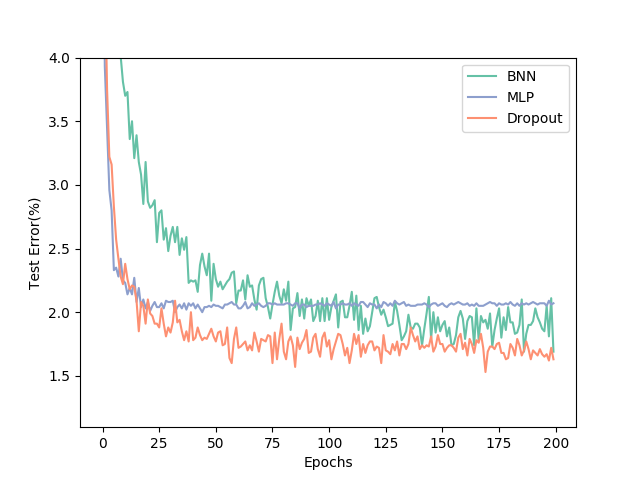
\includegraphics[width=.45\textwidth]{figures/test_error_compare.png}
  \centering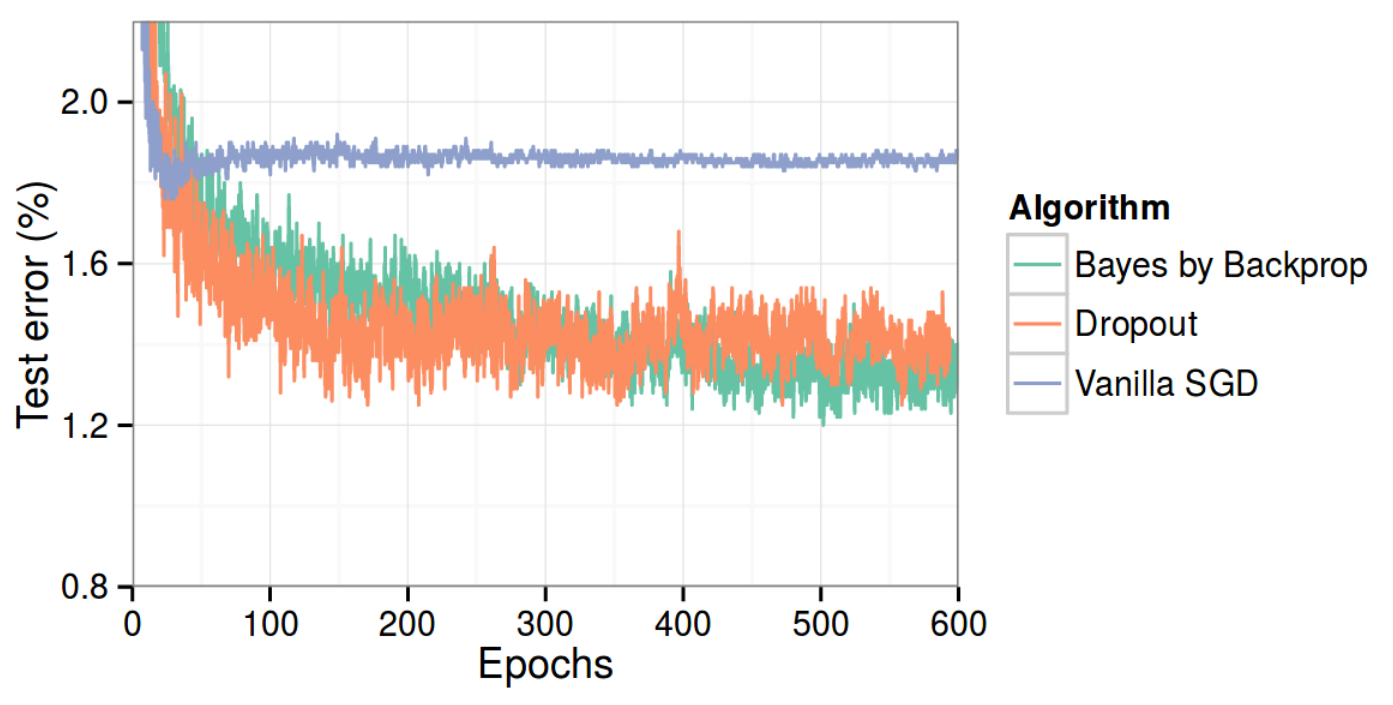
\includegraphics[width=.45\textwidth]{figures/test_error_compare_paper.png}
  %
  \caption{Left: Test error on MNIST using our implementation (2-layers of 400 units).
  Right: Test error on MNIST as detailed in~\cite{blundell} (2-layers of 1200 units).}
  \label{fig:mnist_test_error}
  %
\end{figure}
 

\paragraph{Results}

The first experiment we preformed was simply to train and test our BNN on the
MNIST dataset and compare the results to that of~\cite{blundell}. This allowed
us to ensure that our implemenation of both the BNN and the simple MLPs were
correct and got comparable results. \Cref{fig:mnist_test_error} shows the
test error for the three different models detailed above: a BNN, a standard
MLP, and a MLP with dropout. While our results are not identical to those of
Blundell et al.\, they are very similar. 

In both plots the vanilla MLP is the first to converge and then hovers around
the same test error for the rest of the training epochs. Both the MLP with
dropout and the BNN eventually get a lower test error than the standard MLP
with our BNN taking a significant amount more time than the BNN
in~\cite{blundell}. This along with the overall lower test error in the plot
from~\cite{blundell} can be explained due to the original work using cross
validaton to opimize the hyperparameters whereas our hyperparameters are
certainly not optimal. The last thing of note here, is that while out BNN never
got a lower test error than that of the MLP with dropout, Blundell et al. had
to run their BNN for $400$ epochs before this occured. As our BNN showed no
sign of overfitting at $200$ epochs we can expect it would eventually out
preform the MLP with dropout given enough time.

In our next experiment we wanted to ensure that the BNN was actually learning 
a distribution for each weight in the network and was not simply converging to
a mean value with a standard deviation close to zero. In order to do this we
collected the weights for all the units in the networks, sampling weights 
from the variational posterior in the BNN and using the test weights for the 
MLP with dropout, and then created the density histogram in
\cref{fig:mnist_weight_density}. From this histogram we can see that our BNN
has both the widest range of weights and also the least weights centered at
zero when compared to the two other models. This confirmed that the BNN was
learning a distribution over weights and also confirmed that our 
implementation was correct as it closely mimics the result in~\cite{blundell}.

\begin{figure}
  %
  \centering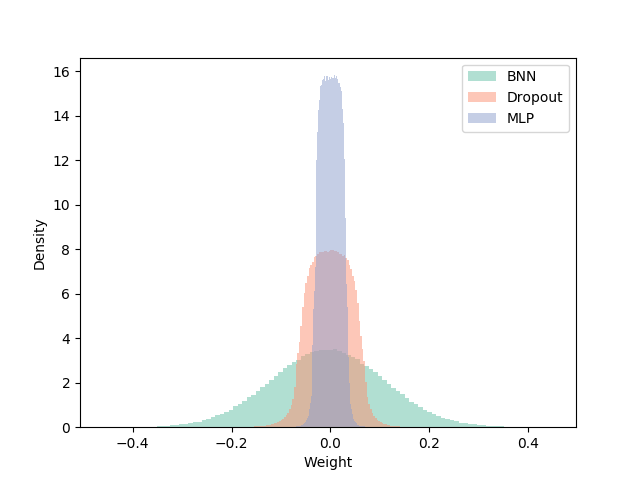
\includegraphics[width=.6\textwidth]{figures/weight_density_compare.png}
  %
  \caption{Histogram of the trained weights of the three types of network we
  compared in \cref{fig:mnist_test_error}}
  \label{fig:mnist_weight_density}
  %
\end{figure}

\subsection{Regression --- Synthetic Data}
Moving on from classification, we wanted to ensure that our BNN implementation 
was able to work on a regression task in addition to the classification task
detailed above. Once again following the work done in~\cite{blundell}, we 
generated training data from the following non-linear function:
\begin{align*}
  y = x + 0.3 \sin(2\pi (x &+ \epsilon)) + 0,3 \sin(4\pi (x + \epsilon)) + \epsilon \\
  \epsilon &\sim \mathcal{N}(0, 0.02)
\end{align*}
\Cref{fig:reg_syth_data} shows this function both with and without noise.
Note that we only generated data in the range $x\in [0, 0.5]$.

\begin{figure}[H]
  %
  \centering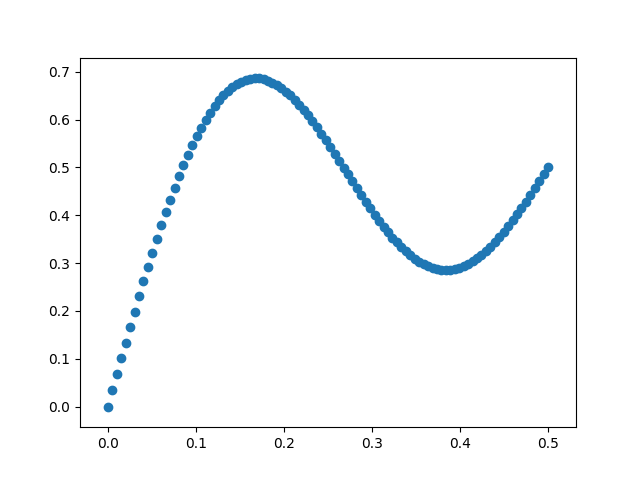
\includegraphics[width=.45\textwidth]{figures/regression_curve.png}
  \centering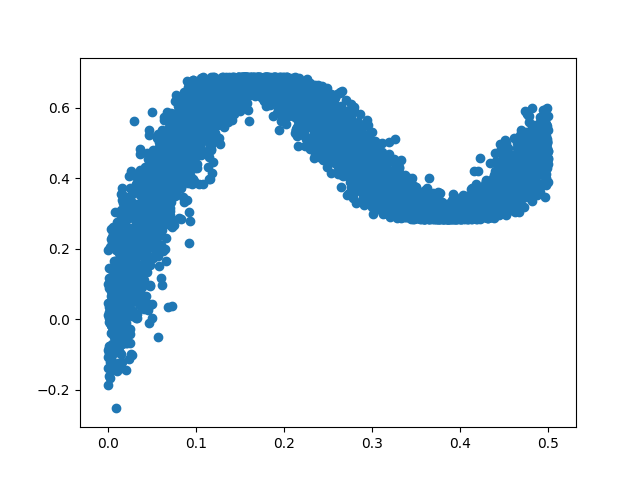
\includegraphics[width=.45\textwidth]{figures/regression_curve_with_noise.png}
  %
  \caption{Left: Noise free non-linear function we generated test data from.
  Right: Noisy non-linear function we used as training data.}
  \label{fig:reg_syth_data}
  %
\end{figure}

\paragraph{Results} 

We trained two different networks on the synthetic data detailed above: our BNN
and a simple MLP without dropout. Both of these networks consisted of
two-layers of $100$ ReLUs and were trained using SGD to minimize L1 loss.
\Cref{fig:reg_extended} shows the functions generated by these two networks
once they were trained for $50$ epochs. We can see from this figure that the
MLP will always predict the same output over mutliple test runs whereas the BNN
has a range of possible outputs. It is important to note here that while both
networks were able to fit the function well in the area where the was training
data, between $x=0.0$ and $x=0.5$, the MLP makes the assumption that the data
outside this range will follow the training data whereas the BNN prefers to
allow many possible extrapolations. This experiment nicely illustrates our
earlier point that a standard neural network can be overly confident about the
uncertainity in the training data whereas our BNN is able to realize it is
unsure about the value of the function outside the training data and perfers to
let the function wander.

\begin{figure}
  %
  \centering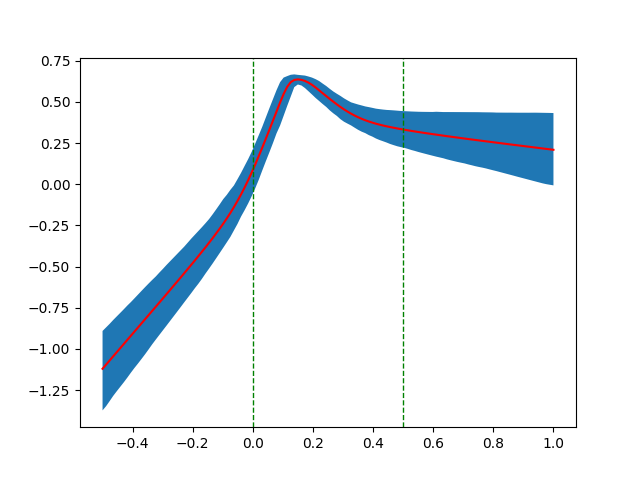
\includegraphics[width=.45\textwidth]{figures/reg_bnn_extended.png}
  \centering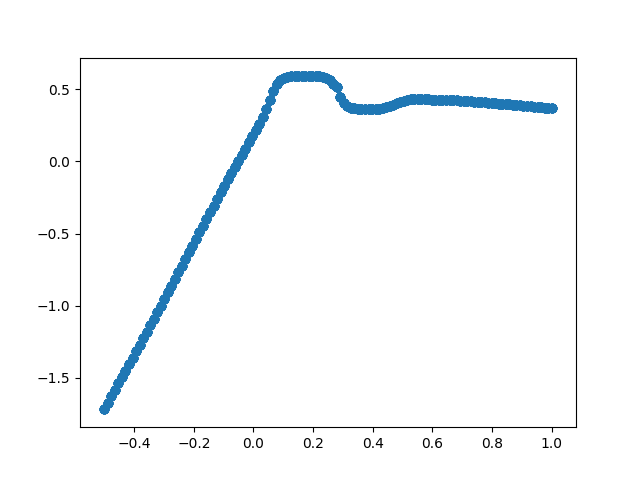
\includegraphics[width=.45\textwidth]{figures/reg_mlp_extended.png}
  %
  \caption{Regression on noisy non-linear function with interquatile ranges.
  Red lines are the median predictions and blue areas are the interquantile range.
	The dotted greeen lines indicate the range of x-values from which the training
  data was generated.
  Left: BNN, Right: MLP.}
  \label{fig:reg_extended}
  %
\end{figure}

\subsection{Contextual Bandits}

Contextual Bandits (CB) are a standard problem from the field of reinforcement
learning which can be interpreted as either an extension of Multi-Armed Bandits
(with the introduction of contexts/states), or a restriction of fully
observable Markov Decision Processes (without the agent's ability to influence
the context/state generative process).  A CB agent iteratively receives
a \emph{context} $\bm x\in\mathcal{X}$, and is subsequently prompted to select an
\emph{action} from a predefined set $\bm a\in\mathcal{A}$.  The agent then receives
a real \emph{reward} $\bm r\in\mathbb{R}$ sampled from an unknown stationary
distribution $\bm r\sim P(\bm r\mid \bm x, \bm a)$, before receiving a new
independent context and repeating the process for a given (potentially
indetermined) amount of time steps.  The goal of the agent is that of
maximizing the long term average of all the received rewards $\Exp\left[\bm
r\right]$.  

Agents typically start out with very limited prior knowledge concerning the
process dynamics (the context or reward distributions).  As a consequence, good
strategies for the maximization of the long-term expected rewards necessarily
involve the (locally sub-optimal) sub-goal of gathering more information about
the process itself.  This notion is know as the \emph{exploration/exploitation}
trade-off, and is a fundamental principle which will determine the success of
a CB agent.  Viewing CB agents from the perspective of how they implement the
exploration/exploitation trade-off, we can roughly split them into three
categories:
%
\begin{description}
  %
  \item[Non-Bayesian ---]  This type of approach learns a point-estimate of the
    expected return associated with the context-action pair $(\bm x, \bm a)$.
    These methods learn to model the information necessary for exploitative
    purposes, but inherently lack the means to implement an explorative
    strategy.  As a consequence, they are paired with an independent
    explorative strategy (typically $\epsilon$-greedy) which occasionally
    selects random actions.
  %
  \item[Bayesian (Optimal) ---]  This type of approach learns a model of the
    full conditional distribution $P(\bm r\mid \bm x, \bm a)$, and uses it to
    implement long-term optimal strategies which plan multiple steps ahead.
    While this approach typically obtains the best performance, it is also the
    hardest to define and implement.
  %
  \item[Bayesian (Heuristic) ---]  This type of approach also requires
    a conditional model over rewards, but implement simpler action-selection
    strategies which, albeit still dependent on the model's learned uncertainty,
    provide fewer guarantees compared to Basyesian-optimal strategies.  
  %
\end{description}

Conditioned on the fact that the model uncertanties are appropriately learned,
non-optimal Bayesian approaches typically perform better than non-Bayesian ones
due to the fact that the exploration rate becomes dependent on the model
uncertainty (rather than constant) and that the exploration targets the more
promising actions (rather than being uniform across all of them).

To demonstrate the fact that the uncertainty learned by Bayes-by-Backprop is
appropriate for a pluritude of tasks, the authors propose to use Thompson
sampling---one of the simplest yet most effective Bayesian non-optimal
approaches---to showcase that the resulting agent's performance is better than
other standard non-Bayesian approaches.  In Thompson sampling, each action is
selected with the same likelihood that it is the optimal action under the
current reward model\footnote{Note that, while Thompson sampling is a very
sensible approach, it is \emph{not} a Basyesian optimal strategy due to the
fact that exploration is a byproduct of the model uncertainty, rather than an
explicit consideration made to maximize long-term returns.}.  

\todo[inline]{Move thompson inside bayesian heuristic paragraph?}

\paragraph{Data --- Mushroom Domain} The Mushroom Data Set~\cite{mushroom}
contains 8124 instances corresponding to 23 species of North American mushrooms
described in terms of 23 discrete attributes, one of which indicates whether
the mushroom is toxic or edible, and the other 22 of which are related to their
shape, size, color, population, habitat, etc.

The context is created by concatenating the one-hot encoding of the 22
attributes, resulting in a context $\bm x\in \{0, 1\}{}^{117}$.  The binary
variable $\bm y\in\{0, 1\}$ is used to denote whether the mushroom is edible,
whereas the action set $\mathcal{A} = \{0, 1\}$ indicates whether the agent
will eat the mushroom.  The rewards are produced as follows (Note that, while
it is possible to obtain a better reward by eating a toxic mushroom due to
luck, in average it is better to avoid it.)

\begin{center}
\begin{tabular}{ccl}
  $\bm y$ & $\bm a$ & $\bm r$ \\ 
  \toprule
  --- & avoid & $0$ (Deterministic) \\
  edible & eat & $5$ (Deterministic) \\
  toxic & eat & Categorical\@($\{5, -35\}$; $p=\{0.5, 0.5\}$) \\  
\end{tabular}
\end{center}

In this experimental setup, the authors train a NN on the regression problem of
predicting the expected reward corresponding to a context-action pair $(\bm x,
\bm a)$.  
Because a BNN trained via Bayes-by-Backprop provides
uncertainty measures, the proposed model is paired with Thompson sampling,
while the baselines consist of standard NNs, trained via Backpropagation, and
paired with greedy, $.05$-greedy and $.1$-greedy action-selection strategies.


\paragraph{Results} 

The performance of a CB agent can be measured in terms of how much
\emph{regret} it accumulates over time.  The regret corresponding to a single
interaction is defined as the difference between the obtained reward, and the
reward which would have been obtained by an oracle who knows the mushroom's
toxicity.  In this domain, the oracle would always eat an edible mushroom
(receiving reward $5$), and always avoid a toxic one (receiving reward $0$).
The resulting regret function is:
%
\begin{equation}
  %
  \operatorname{Regret}(\bm r, \bm y) = \bm r - 5 \, \Ind\left[ \bm
  y = 1 \right]
  %
\end{equation}

\Cref{fig:cb_cumregret} depicts the cumulative regrets obtained by the
non-Bayesian CB agents and the one trained with Bayes-by-Backprop.  

While we were able (with a caveat, explained soon) to implement the
non-Bayesian agents and confirm similar results as those reported in
\cref{fig:cb_cumregret}, we were unfortunately unable to do the same for the
Bayesian agent trained via Bayes-by-Backprop.

\todo[inline]{Finish caveat and description}


\begin{figure}
  %
  \centering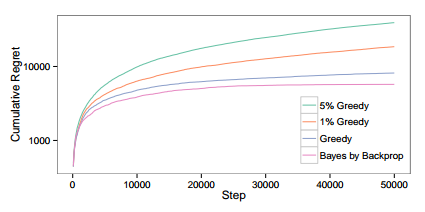
\includegraphics[width=.5\textwidth]{figures/cb_cumregret.png}
  %
  \caption{Cumulative regret obtained by non-Bayesian CB agents, and the BNN
  agent trained via Bayes-by-Backprop.  Figure taken directly
  from~\cite{blundell}.}\label{fig:cb_cumregret}
  %
\end{figure}


\section{Conclusions}

In recent decades, Neural Networks have proven themselves as a very successful
model choice for a wide variety of regression tasks on diverse data sets.
Arguably, this is due to the inherent feature representation learning performed
by the hidden layers (when trained well).  Compared to other advanced ML models,
one aspect where standard NNs are suboptimal is the virtual infeasibility of
a complete Bayesian treatment of inference, regression or prediction.  The high
number of model parameters and the complex nature of the dependencies between
parameters in different layers are both factors which render a precise joint
Bayesian treatment of the model weights not tractable.

The main contribution of Blundell et al.\ is the proposal to use
state-of-the-art approximate inference to extend NN model usage, and an
extension of the most common training principle (gradient descent via
backpropagation) for such purpose.  The proposed BNN model is tested on
multiple tasks, including classification, regression and reinforcement
learning.  The presented results support the claim that the model uncertainties
are adequately learned and that BBVI is a feasible way to perform approximate
Bayesian inference with NN models; The mild success that we've had in
replicating these results gives further credit to their claims.

The proposed training framework is in essence a combination of multiple
well-established ML principles, and as such it respectively enjoys and suffers
from their known advantages and pitfalls: Backpropagation is very sensitive to
hyperparameters, and generally suffers from convergence to multiple local
optima; SGD allows the training to handle much bigger data sets than the
non-SGD version of NN training; The MC estimation of the gradients can be
parallelized straightforwardly, thus reducing (given sufficient hardware
resources) the absolute training time required; Finally, VI increases the
number of training parameters, which also impacts the number of training
iterations typically necessary to convergence.


\bibliographystyle{plain}
\bibliography{references} 

\end{document}
